% This is LLNCS.DOC the documentation file of
% the LaTeX2e class from Springer-Verlag
% for Lecture Notes in Computer Science, version 2.4
\documentclass{llncs}
\usepackage{llncsdoc}
\usepackage[noend]{algpseudocode}
\usepackage{subfig} 
\usepackage{graphicx}
\usepackage{frame, caption}
\usepackage{amsmath}
\usepackage{eulervm}
\usepackage{fontenc}
\usepackage{mathrsfs}
\usepackage{multirow, enumitem, longtable, rotating,lipsum, scrextend}
\usepackage{array}
\usepackage{floatflt}
\usepackage{makecell}
\usepackage{xcolor, soul}
\sethlcolor{yellow}	
\usepackage{floatrow}
\usepackage{setspace}
\newcommand{\argmax}{\operatornamewithlimits{arg\,max}}
%
\begin{document}
	\title{\vskip -10pt A computational model of power in collaborative negotiation dialogues}
	
	\author{Lydia Ould Ouali\inst{1},  Nicolas Sabouret\inst{1}\and
		Charles Rich\inst{2} }
	
	\institute{LIMSI-CNRS, UPR 3251, Orsay, France \\
		Universit\'e Paris-Sud, Orsay, France \\
		\email{\{ouldouali, nicolas.sabouret\}@limsi.fr}
		\and
		Worcester Polytechnic Institute\\ Worcester, Massachusetts, USA\\
		\email{rich@wpi.edu}
	}
	
	\maketitle
	
	\begin{abstract}
		This paper presents a conversational agent that can deploy different strategies of negotiation based on its social power. The underlying computational model is based on three principles of collaborative negotiation from the literature in social psychology. The social behavior of the agent is made visible through its dialogue strategy. We evaluated our model by showing that these principles are correctly perceived by human observers on synthetic dialogues.
	\end{abstract}
	
	\section{Introduction}
	
	As they rise in popularity, artificial conversational agents become more present in daily applications in which they play different roles such as pedagogical robots, companion robots for children or for the elderly, etc. In these situations, agent and user have to collaborate through their interaction in order to achieve shared goals. Such example of collaboration can be found in intelligent tutoring agents \cite{kerly2008calmsystem}, where agent and learner collaborate to achieve exercises. They compare their respective knowledge on the problem to be solved and discuss possible solutions. Such confrontation offers a personalized teaching to the learner.
	
	As illustrated in the above example, user and the agent typically negotiate in a collaborative manner about the way to achieve the shared goal, depending on individual expertise and preferences. This specific type of discussion is called \emph{collaborative negotiation}. Unlike adversarial negotiation \cite{broekens2010affective}, collaborative negotiation assumes that each participant is motivated by the goal of finding a trade-off that best satisfies the interests of both participants, instead of one that maximizes his own interest \cite{sidner1994artificial,chu1995response}.
	%For instance,  CALMsystem \cite{kerly2008calmsystem} turoring agent presents the learner with their learner model, offering them the opportunity to compare their own beliefs regarding their capabilities with those inferred by the system, and allow the learner to negotiate over the proposed representations.
	
	Our goal is to build conversational agents capable of credible collaborative negotiation with a human user. To this end, we need to understand how human beings behave in such situation. Indeed, as stated by \cite{broekens2010affective}, negotiation is a multifaceted process which involves social interaction and affects as well as personal preferences and opinions. Therefore, it is crucial to understand the impact of social aspects of the negotiation process. Researchers in social psychology and communication \cite{dunbar2005perceptions,de1995impact} showed that \emph{social power} directly  affects the strategies of negotiators. Therefore, we claim that conversational agent which is able to negotiate with a user must be able to adapt their negotiation strategies to different levels of power.
	
	In this paper, we present a conversational agent that aims to contribute to essentials aspects of conversation agents in terms of negotiation and social behaviors. We propose an agent capable of negotiating with the user. In addition, it can deploy different strategies of negotiation based on the social power it wants to express.
	
	In the next section, we discuss existing works on interpersonal power in the domain of social psychology and affective computing. Section 3 presents the computational model of negotiation, based on a set of utterance types and a model of preferences. It implements a general model of negotiation based on three principles of collaborative negotiation from the literature in social psychology. In section 4, we present an experiment conducted with two virtual agents on a negotiation about restaurants showing that the principles are correctly perceived by human observers.	
	
	\section{Related work}
	The notion of social power has been widely studied in the fields of interpersonal communication and psychology \cite{kecskes2013research}. It can be defined as the capacity to produce intended effects and to influence the behavior of the other person in the conversation \cite{dunbar2005perceptions}. In the context of communication and negotiation, power is a dyadic variable that takes place during the dialogue.
	%, where the interlocutor who exerts power is viewed as \textit{dominant}, while the interlocutor with low power's behaviors is viewed as \textit{submissive}. 
	% where one individual's attempt of control is necessarily acquainted by the partner in the interaction.\cite{dunbar2005perceptions
	Behaviors related to power can contribute either positively or negatively to the dialogue. Positive contributions include keeping the conversation going and making quick decisions. Negative contributions include not considering the partner (\emph{e.g.} not giving the occasion to express his opinion) and appearing offensive. In our work, we focus on negotiation dialogues, in which several researchers have already shown the impact of social power\cite{de2004influence,burgoonnonverbal}.
	
	\subsection{Behaviors of power in dialogue}
	\label{sec:domDialogue}
	During a dialogue, power can manifest through verbal and nonverbal behaviors.	
	At the nonverbal level, a wide range of behaviors have been associated with the relation of power in kinesthetic behaviors (facial expression, body movements and gestures) and voice (speaking duration, speaking intensity, voice control and pitch) \cite{burgoonnonverbal}. Based on this work, several conversational agents have been developed with the ability to exhibit social power through nonverbal behavior, such as gaze \cite{lance2008relation}, body movements \cite{mignault2003many} or head tilt \cite{gebhard2014exploring}
	%,callejas2014computational}
	in relation to high-power and low-power perception.
	
	However, power is also expressed through verbal behaviors. A considerable body of research in social science and communication has documented the effects of power on negotiation behaviors and outcomes. De Dreu \cite{de1995impact} demonstrated that high-power negotiators have higher aspirations, demand more and concede less. Galinsky \cite{galinsky2003power} affirms that power increases the action orientation: high-power negotiators control the flow of the negotiation. In addition, high power increase task orientation and goal-directed behavior. Giebels \cite{giebels2000interdependence} shows that this leads powerful negotiators to end up with the larger share of the pie.
	
	Furthermore, power affects the way that negotiators gather information about their partners \cite{de2004influence}. Low-power negotiators have a stronger desire to develop an accurate understanding of their negotiation partner, which leads them to ask more \emph{diagnostic} rather than \emph{leading} questions.
	
	It was also shown that high-power negotiators are self-centered and tend  not to pay attention to the preferences of the less powerful negotiators \cite{fiske1993controlling,de1995impact}.
	%					 The idea is that high-dominant individuals have many resources and can often act at will without serious consequences, while submissive individuals, have to be more careful because they are more dependent on other people. In addition, they are motivated to gain or regain control over their outcomes by paying close attention to the people on whom they depend.
	%					
	
	%In our work, we use a text-oriented dialogue system and we therefore focus on the verbal behaviors. 
	Our goal is to develop a model of dialogue for Virtual Agents which considers these properties related to social power. We want to make visible \emph{the strategies} deployed during the negotiation depending on the power. In order to implement these different behaviors, we identified three principles related to the relation of power and their impact on the strategy of negotiation
	\begin{enumerate}
		\item \textbf{Level of demand and concession:} High-power negotiators show a higher level of demand than the low-power ones. In addition, low-power negotiator's demand decrease over time and the negotiator tends to make larger concessions than high-power negotiators. \cite{de1995impact}
		
		\item \textbf{Self vs other:} Low-power negotiators consider the preferences of the other in the negotiation, whereas high-power negotiators are self-centered and only interested in satisfying their own preferences. \cite{fiske1993controlling,de1995impact}
		
		\item \textbf{Controlling the flow of the negotiation:}
		High-power negotiators tend to make the first move \cite{magee2007power} and take the lead in the negotiation. Low-power negotiators aim to construct an accurate model of other preferences, which leads them to ask more questions about other preferences rather than keeping the negotiation going (\emph{e.g} by making proposals)\cite{de2004influence}. 
		
	\end{enumerate}
	
	In the context of collaborative negotiation, we must combine these principles with the goal of finding a trade-off that satisfies both negotiators.
	
	
	%	We will present in the next section the decision model based on the behaviors of power. 
	%						\item Based on Carsten, De Dreu and Van Kleef demonstrate that high power negotiators are high in their propensity to negotiate relative to participants with low power. (leading individuals to focus on the rewards available to them in situations and to bargain forgreater rewards than were initially offered to them.)
	\subsection{Similar work in the literature}
	Only a few researchers have considered the expression of power in the verbal behavior of a conversational agent. \cite{bee2010bossy} developed an agent that expresses social power through gaze and linguistic features. They demonstrated that linguistic personality traits influence the perception of power. However, this work does not consider how power affects the strategies of negotiation in dialogue. More recently, \cite{broekens2010affective,de2015humans} consider trust, expression of emotions as anger and happiness as dimensions of the negotiation strategy of a virtual agent. However, this research focuses more on the negotiation aspect than on the expression of social power. In our work, we want to investigate the expression of power through the dialogue strategy, which has not been considered by previous work.
	
	In a different context, \cite{nazari2015opponent} studied how the communication of preferences in a negotiation with a human can impact the negotiation outcomes. They consider situations in which negotiators can use deception to gain an unfair advantage and can hide their intentions. We do not consider this case in our work. Our agents are not only collaborative, but they also give correct information about their preferences and they do not try to hide any information. Previous work such as \cite{swartout2006toward} showed that, even in collaborative negotiation, it is not always possible or advisable to give information about all preferences.
	
	\section{Model of negotiation based on the relation of power}
	In this section, we present our model of dialogue for a Virtual Agent  in the context of collaborative negotiation based on power.	
	First, we present the data structure for the agent's preferences and the topics of the negotiation. Second, we present the implementation of the principles of behaviors of power in negotiation discussed in this section \ref{sec:domDialogue}.
	\vspace{-1em} 
	\subsection{Domain model}
	The overall goal of a negotiation is to choose an \textbf{option} in a set of possible options $\mathcal{O}$. The evaluation of each option by participants is based on a set of \textbf{criteria} that reflect the option's characteristics. Let us consider a set $\mathcal{C}$ of $n$ criteria and let $C_1,\ldots,C_n$ be their respective domains of values. $\mathcal{O}$ can be simply defined as the cross-product $C_1\times\ldots\times C_n$ and each option $o\in\mathcal{O}$ is a tuple $(v_1,\ldots,v_n)$, making the simplifying assumption that all options are available. For instance, in a dialogue about restaurants, the criteria might be the type of cuisine and the price, we could have the option: $(French,expensive)$.
	
	\subsection{Preference model} 
	The conversational agent is defined with a set of preferences, formalized as a set of partial orders $\prec_i$ on each $C_i$. For instance, if the agent prefers French food to Italian, $Italian\prec_{cuisine}French$.
	
	For a given criterion $i\in \mathcal{C}$, for a given value $v\in C_i$, the agent computes its \emph{satisfaction} $sat_{self}(v \prec_i)$ for this value as the number of values it prefers less in the partial order $\prec_i$, normalized in [0,1]:
	\vspace{-.5em} 
	\begin{equation}
	sat_{self}(v, \prec_i) =	1 - \left( \frac{|\{v' : v' \neq v \  \wedge \ (v \prec_i v')\}| }{( |C_i| - 1 )}\right)
	\end{equation}
	
	This notion of satisfaction is generalized to any option $o= (v_1, \ldots, v_n)\in \mathcal{O}$ as a simple average\footnote{There exists a great amount of literature in theoretic decision making on how to combine multiple criteria using Order Weight Averages or Choquet's integrals, for instance. We are not concerned with this question of criteria aggregation in this paper.}:
	\vspace{-1em} 
	\begin{equation}
	sat_{self}(o, \prec) = \frac{\sum_{i=1}^{n} sat_{self}(v_i, \prec_i) }{n}
	\vspace{-1.5em} 
	\end{equation}
	
	\bigskip
	The satisfaction represents the tendency for an agent to accept or to propose a possible value or option in the negotiation dialogue: the closer to 1, the more it will be selected early in the negotiation.
	
	\subsection{Dialogue model}
	Negotiators communicate during the negotiation via \emph{utterances}. Each utterance type has a specific set of arguments and is associated with a specific expression in natural language (NL). We use five utterance types, based on the work of Sidner \cite{sidner1994artificial} and two additional utterances to close the negotiation. Table \ref{table:utt} summarizes these generic utterance types. Only the NL generation of these utterances has to be specialized in the application domain. In this paper, we will illustrate this model on a collaborative negotiation about restaurants. The value /$v$/ in Table \ref{table:utt} refers to this NL format to express a value.
	%, and three derivate types that are combinations of the main ones.
	% changer le tableau, enlever parametre comme tab2 et ajouter les ensembles de valeurs a la fin	
	
	Each utterance type takes as parameter either a criterion value $v \in C_i$, an option $o \in \mathcal{O}$ or a criterion type $i \in \mathcal{C}$. They can be separated into three groups. Information moves (\textit{AskValue/AskCriterion} and \textit{StateValue}) are used to exchange information about the participant's likings. In human-human negotiation dialogue, we observed that partners tend to express what they like or do not like (\emph{e.g} \textit{I (don't)like Chinese restaurants})  rather than binary comparison (\emph{e.g} \textit{I like Chinese more than French}). This is the reason we use unary operators for the information utterances.
	
	Negotiation moves (\textit{Propose}, \textit{Accept} and \textit{Reject}) allow the agent to make or to answer to proposals. The agent can propose, accept and reject both values (``Let's go to a Chinese restaurant'') or options (``Let's go to \emph{Chez Francis}'').
	
	Closure moves (\textit{NegotiationSuccess} or \textit{NegotiationFailure}) are used to end the dialogue.
	%The RejectPropose utterance type is used to clearly reject an option and make a counter-proposal in the same dialogue move. Similarly, the RejectState utterance type is used to make a reject with an explanation. The AcceptPropose is used to accept a criteria and propose a compatible option. 
	Examples of dialogues for restaurants are given in section \ref{sec:evaluation}.
	
	\medskip
	The decision process for utterance selection is based on our three principles and is described in section \ref{sec:decision}. To perform this utterance selection, the agent keeps track of all statements and proposals during the dialogue. For each criterion $i\in\mathcal{C}$, we build the set $S_i \subseteq C_i$ of statements that the agent has made about this criterion. This avoids restatements of previous information. We also build the sets $A_i\subseteq C_i$ and $U_i\subseteq C_i$ of values which have been stated by the interlocutor as liked or disliked through \emph{StateValue} utterances. We assume that $A_i\cap U_i=\emptyset$.
	
	We also maintain the sets $P_i \subseteq C_i$, $T_i\subseteq C_i$ and $R_i\subseteq C_i$ of all proposed, accepted and rejected values for each criteria. These will be used to make relevant proposals. Similarly, we consider $P\subseteq \mathcal{O}$, $T\subseteq \mathcal{O}$ and $R\subseteq \mathcal{O}$ the sets of all proposed, accepted and rejected options in the dialogue.
	
	\begin{table}[t]
		{\scriptsize
			\begin{tabular} {|p{2.75cm}|p{4cm}|p{3cm}|}
				\hline
				\textbf{Utterance type}  &\textbf{ NL generation} & \textbf{Postcondition}\\
				\hline
				StateValue(v) &  I (don't) like /$v$/. & Speaker : $v \in S_i$ \newline Hearer:  \newline $v\in A_i$ is likable, $v\in U_i$ otherwise \\
				\hline
				AskValue(v)& Do you like /$v$/ ? & \multirow{2}{*}{} \\
				
				AskCriterion(i) &  What kind of /$i$/ do you like ? & \\
				\hline
				ProposeOption(o)  & Let's go to /$o$/. & $o \in P$\\
				
				ProposeValue(v) & Let's go to a /$v$/. & $v \in P_i$\\
				\hline
				AcceptOption(o)& Okay, let's go to /$o$/.& $o \in T$ \\
				
				AcceptValue(v) & Okay, let's go to a /$v$/.& $v \in T_i$ \\
				\hline
				RejectOption(o) & I'd rather choose  something else. & $o \in R$\\
				
				RejectValue(v) &  I'd rather choose  something else. & $v \in R_i$ \\
				\hline
				NegotiationSuccess &  We reached an agreement. & \multirow{2}{*}{}\\
				\cline{1-2}
				NegotiationFailure &  Sorry, but I no longer want to discuss this. & \\
				\hline
				% Counter Propose & $(r,p)\in C_i^2 \vee (r,p) \in \mathcal{O}^2 $ & I don't want to go to $r$. Let's rather go to $p$ \\
				% \hline 
				% RejectState & $x \in \mathcal{O} \vee x\in C_i$ &  I don't like /$x$/, let's choose something else. \\
				% \hline
				% AcceptPropose & $o \in \mathcal{O}$ & Okay. Let's go to /$o$/.\\
				% \hline
			\end{tabular}
		}
		\caption{\label{table:utt}List of utterance types in the model of dialogue.}
	\end{table}
	
	\subsubsection*{Satisfiability}
	Using the sets $A_i$ and $U_i$ that represent the interlocutor's likings, the agent can compute the satisfiability of a value $v\in C_i$ for the interlocutor (\emph{i.e.} the \emph{other} person) using the following formula:
	\vspace{-0.5em} 
	\begin{equation}
	sat_{other}(v)= \left\{\begin{array}{ll}
	1	 & \mathrm{if\ }  c \in A_i\\
	0    & \mathrm{if\ }c \in U_i\\
	0.5	 & \mathrm{otherwise}
	\end{array}\right.
	\end{equation}
	
	%...
	Note that some values might remain unknown: in a collaborative negotiation, they can be considered as being potentially satisfiable. Therefore, we give them an arbitrary value fixed to $0.5$.
	
	This function is generalized to any option $o=(v_1,\ldots,v_n) \in O$:
	
	\begin{equation}
	sat_{other}(o, A, U) = \frac{ \sum_{i}^{n} sat_{other}(v_i, A_i, U_i) } {n}
	\end{equation}
	
	The satisfiability represents the expectation an agent has about the other accepting or rejecting a proposal. It will be used to select the most tolerable offer to make in the negotiation. The concept of tolerable is presented in the next section.
	
	\subsection{Decision based on power in negotiation}
	\label{sec:decision}
	
	In section \ref{sec:domDialogue}, we identified three principles related to the relation of power which affects negotiators strategies and behaviors. In this section, we present the computational theory implementing each principle. 
	
	We denote the agent's belief of its  power $pow \in [0, 1]$. It is a constant for a given agent in a given interaction.
	
	
	\subsubsection{Level of demand and concession}
	
	In collaborative negotiation, both participants reduce their level of demand over time because they want to reach an agreement. However, according to our first principle, the level of demand should be higher for high-power agent and concessions should be greater for low-power ones. To model this behavior, we use a \emph{concession curve} illustrated in Figure \ref{fig:conc}.
	
	Let $self(pow, t)$ be a time varying value, following the concession curve:
	\begin{equation}
	self(pow, t) = \left\{\begin{array}{ll}
	pow & \mathrm{if\ } (t \leq \tau)\\
	max(0, pow - (\frac{\delta}{pow} \cdot (t - \tau))) & \mathrm{otherwise}
	\end{array}\right.
	\end{equation}
	\begin{floatingfigure}[r]{1.8in}
		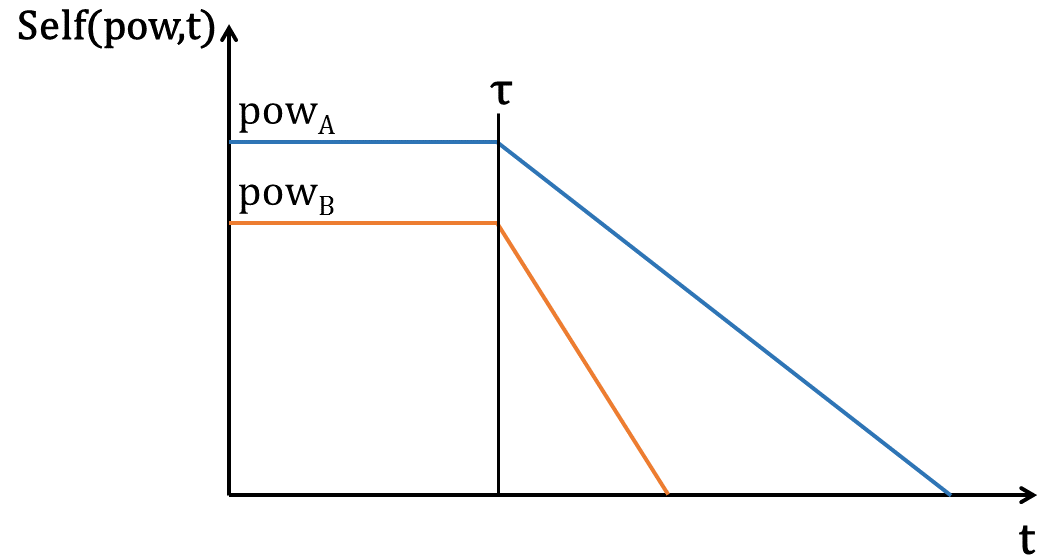
\includegraphics[width=1.8in]{graphs/sv3.png}
		\caption{\label{fig:conc}Concession curve}
	\end{floatingfigure} 
	where is $t \geq 0$ is the number of open or rejected proposals, $\tau > 0$ is the minimum number of proposals before the concession begins and $\delta > 0$ is a computational parameter of the concession slope.
	
	The value $self(pow,t)$ represents the weight an agent gives to its self-satisfaction relative to the satisfaction of its partner. The higher the agent's power gets, the higher its demands get. In addition, the slope decreases faster for low values of power.
	
	These behaviors of demand and concession are implemented in the computation of an \textit{acceptability} value. Based on the value of satisfiability, the agent is able to tell if it likes a value or not.
	
	The acceptability of a value $v \in C_i$ is defined as a boolean function:
	\begin{equation}
	\vspace{-.5em} 
	acc(pow,v, t) = sat_{self}(v, \prec_i) \geq  (\beta \cdot self(pow,t))
	\end{equation}
	
	\medskip
	where $\beta>0$ is a parameter of the theory that defines the weight given to the level of demand.
	
	This boolean function is generalized to any option $o \in O$: $acc(pow,o, t) = sat_{self}(o, \prec) \geq  (\beta \cdot self(pow,t))$. This acceptability is used by the agent to decide whether he accepts a proposal or not.
	
	
	\subsubsection {Self vs other}
	According to our second principle, high-power negotiators give more weight to their own satisfaction. To implement this principle in the context of collaborative negotiation, we compute how much a given proposal is \emph{tolerable} considering the satisfiability for both the agent and its partner.
	% The value returned by $tol$ is used to build proposals during the negotiation. 
	
	For a given criteria $i\in\mathcal{C}$, let us consider the subset $V_i\subseteq C_i$ of values that are acceptable for the agent:
	\vspace{-0.5em} 
	\begin{equation}
	V_i(pow,t) = \{ v\in C_i : acc(pow,v,t) \}
	\vspace{-0.5em}
	\end{equation}
	This set corresponds to all the proposals an agent could make at a time of the negotiation.
	
	We compute the tolerability of a given value $v\in V_i(pow,t)$ by balancing between the agent's preferences and the likings of its partner. We assume that the agent gives a weight to its partner satisfaction which is complementary to its self-satisfaction:
	
	\begin{equation}
	\begin{split}
	tol(v, t, \prec_i, A_i, U_i, pow) & = self(pow, t)  \cdot sat_{self}(v, \prec_i) \\
	& +  (1 - self(pow, t)) \cdot sat_{other}(v, A_i, U_i)
	\end{split} 
	\end{equation}
	
	\noindent
	And we generalize this function to any option $o=(v_1,\ldots,v_n) \in O$:
	
	\begin{equation}
	tol(o, t, \prec, A, U, pow) = \frac{ \sum_{i}^{n} tol(v_i, t, \prec_i, A_i, U_i, pow) } {n}
	\end{equation}
	
	\noindent
	The agent will always propose the most tolerable element in $V_i$:
	\begin{equation}
	propose(V_i, \prec_i,pow) =  \operatorname*{arg\,max}_{v \in V_i} ( tol(v))
	\end{equation}
	
	\subsubsection*{Summary of general parameters }
	\begin{itemize}[noitemsep]
		
		\item $\pi \in $[0,1] : boundary between submissive and dominant used in
		choosing an utterance type
		\item $\beta$:  a value that represents the minimum score that a value has to get to be positively satisfiable to the agent preferences in the negotiation. Note that $\beta = const \times self(dom,t)$.
		\item $\tau > 0$ : the minimum number of open or rejected proposals before concession begins
		\item $\delta > 0$ : parameter in slope of concession curve.
		\item $\alpha> 0$: the maximum number of successive statement moves.
	\end{itemize}
	
	\subsubsection{Controlling the flow of the negotiation}
	According to our third principle, high-power negotiators tend to lead the negotiation. We implemented this principle through the choice of utterance types presented in Table \ref{table:uttChoice}.		
	We defined a threshold $\pi$ to split the spectrum of power in two.
	
	Depending on the power, the previous utterance $u^{-1}$ type and the current dialogue state, the agent selects the first utterance type in Table \ref{table:uttChoice} for which the condition is satisfied. For instance, a high-power agent will stop the negotiation as soon as all the remaining options are unacceptable (line 2). A low-power agent will reject and state a preference, so as to explain why the proposal is not acceptable (line 14). If there is no open proposal, the low-power agent will ask for new information (line 18 -19).
	
	In our model, an agent can express more than one utterance during his speaking turn. This is modeled  with the sign "+" in Table\ref{table:uttChoice}.
	
	Note that a high-power agent will focus on keeping the negotiation going by choosing \emph{negotiation moves} (ProposeValue /ProposeOption, RejectValue /RejectOption, AcceptValue/ AcceptOption) as presented in lines (4 to 10). The agent prioritizes the negotiations moves rather than exchanging information about the preferences. Indeed, as presented in line 3, after $\alpha$  speaking turns dedicated to sharing information, the agent will rather make proposals than stating his likes. An example is presented in the dialogue \ref{fig:ex-dialogue}. 
	
	On the contrary, a lower power negotiator will focus on building an accurate model of its partner's likings in order to take the fairest decision. It will focus more on \emph{information moves} (StateValue or AskValue/ AskCriterion) as seen in line(18-20). Moreover, the negotiation moves are restricted by conditions which ensure that the agent gathered enough information about its partner likes before to express a proposal (line 16-17).
	
	
	\begin{table}[!t]
		{\scriptsize
			\centering
			\begin{tabular}{|p{.3cm}|p{.6cm}|p{3cm}|p{7.5cm}|}
				\hline
				\parbox[t]{2mm}{\multirow{5}{*}{\rotatebox[origin=c]{90}{\textbf{pow  $>\pi$}}}}&Line nb& \textbf{Utterance type} & \textbf{Condition} \\
				\cline{2-4}
				&1&NegotiationSuccess & $\exists o \in T\cup P$, $acc(pow,o,t)$ \\
				\cline{2-4}
				& 2& NegotiationFailure & $ \forall o \in \mathcal{O},  \neg acc(pow,o,t)$\\
				\cline{2-4}
				&3& StateValue(v) & $type(u^{-1}) = AskPreference \land n < \alpha$ \newline where $n$ is the number of successive statement moves\\
				\cline{2-4}
				&4& AcceptValue(v)+ \newline ProposeValue(c) & $ \exists v \in P_i$ / $acc(pow,v,t) \land \exists i\in\mathcal{C}, acc(pow,c,t)$ \\
				\cline{2-4}
				&5& AcceptValue(v)+\newline ProposeOption(o) &  $ \exists v \in P_i$ / $ acc(pow,v,t) \land \exists o \in \mathcal{O}$/ $ v \in o \land acc(pow,o,t)$ \\
				\cline{2-4}
				&6& RejectValue(v)+\newline ProposeValue(c) & $ \exists v \in P_i$ / $ \neg acc(pow,v,t) \land \exists i\in\mathcal{C}, acc(pow,c,t)$ \\
				\cline{2-4}
				&7& RejectValue(v)+ \newline ProposeOption(o) &  $ \exists v \in P_i$ / $  \neg acc(pow,v,t) \land \exists o \in \mathcal{O}$/ $acc(pow,o,t)$ \\
				\cline{2-4}
				& 8&RejectOption($o_1$)+ ProposeOption($o_2$) & $ \exists o_1 \in P$ / $ \neg acc(pow,o_1,t) \land \exists o_2\in\mathcal{O}, acc(pow,o_2,t)$ \\
				\cline{2-4}
				&9& ProposeValue(v) & $\exists v \in C_i$ / $tol(v, t, \prec_i, A_i, U_i, pow)$\\
				\cline{2-4}
				&10& ProposeOption(o) & $\exists o \in \mathcal{O}$ / $tol(o, t, \prec_i, A_i, U_i, pow)$\\
				
				\hline
				
				\parbox[t]{2mm}{
					\multirow{5}{*}{\rotatebox[origin=c]{90}{ \textbf{pow  $ \leq \pi$}}}} & 11& Negotiation success &  $\exists o \in T$ \\
				\cline{2-4}
				&12& AcceptValue(v) & $\exists i\in\mathcal{C}, \exists v \in P_i, acc(pow, v, t)$ \\
				\cline{2-4}
				&13&AcceptOption(o) & $\exists o \in P, acc(pow, o, t)$ \\
				\cline{2-4}
				&14&RejectValue(v)+\newline StateValue(v) & $ t<\tau \land (\exists i\in\mathcal{C}, \exists v \in P_i, \neg acc(pow,v, t))$.\\
				\cline{2-4}
				&15&RejectOption(o)+ \newline StateValue(v) & $ t<\tau \land (\exists o \in P,  \neg acc(pow,o, t) \land \exists v \in o, \neg acc(pow,v, t))$.\\
				\cline{2-4}
				&16&ProposeValue(v) &  $\exists i\in\mathcal{C}, \exists v \in C_i, v \in A_i  \land acc(pow, v, t) $\\
				\cline{2-4} 
				&17&ProposeOption(o)  & $\forall i\in\mathcal{C},\exists v \in C_i, v \in T_i  \land v \in o$ \\
				\cline{2-4} 
				&18&AskValue(v) & $t > \tau \land \exists i\in\mathcal{C}, \exists c \in P_i, \neg acc(c, t)$ \\
				\cline{2-4} 	
				&19&AskCriterion(i) & $\exists i\in\mathcal{C}, A_i \cup U_i= \emptyset $\\
				\cline{2-4}	
				&20&StateValue(v) & $\exists i\in\mathcal{C}, C_i\cap S_i \neq \emptyset$	\\
				\cline{2-4}
				&21& ProposeValue(v) & $\exists v \in C_i$ / $tol(v, t, \prec_i, A_i, U_i, pow)$\\
				\cline{2-4}
				&22& ProposeOption(o) & $\exists o \in \mathcal{O}$ / $tol(o, t, \prec_i, A_i, U_i, pow)$\\
				
				\hline
			\end{tabular}
		}
		\caption{Selection of utterance types}
		\label{table:uttChoice}
	\end{table}
	
	\section{Evaluation}
	\label{sec:evaluation}
	\vspace{-0.5em} 
	In order to evaluate our model, we conducted a controlled study in which participants judge the behaviors of two agents implemented using our model. Our system is written in Java using the DISCO platform \cite{rich09}. This allowed us to produce synthetic dialogues between two artificial agents with different values of power and varying preferences.
	
	\subsection{Study design}
	We simulate a collaborative negotiation for choosing a restaurant using four criteria (cuisine, ambiance, price and location) for a total of 420 options. An example of dialogue is given in the figure \ref{fig:ex-dialogue}. The following parameter values were used in our simulation: $\tau=2$, $\pi=0.5$, $\alpha=2$, $\beta=1$ and $\delta=0.1$. We generated three preferences sets and we measured the difference between the preference sets using Kendall's distance \cite{bra2013Kendall}. We manipulated two simulation parameters: the power of both agents (named \emph{pow-a} and \emph{pow-b}) and the preference sets. This later affects the generation of dialogues in term of values and length.  Table \ref{table:conditions} summarizes the 4 experimental conditions that results from this combination. Note that we only consider one configuration of social power for the similar preference sets condition, because the produced dialogues with other values of power are all very similar in this case. The first speaker (Speaker A) is always the high-power agent, as stated by our third principle of leading the dialogue.
	
	
	Our goal is to show these dialogues to human observers so as to evaluate how the relation of power is perceived in the different dialogues.
	\begin{table}[t]
		\centering
		\begin{tabular}{ |l|c|c|l| }
			\hline
			\textbf{Preferences}& \textbf{A} & \textbf{B} & \textbf{Label} \\ 
			\hline
			\newline\multirow{3}{*} {Different preferences (Kendall's tau = $0.96$)} & 0.9 & 0.4 & Dialogue 1 \\ \cline{2-4}
			
			\newline  & 0.7 & 0.4 & Dialogue 2\\ \cline{2-4}
			
			\newline   &0.7 & 0.2 & Dialogue 3\\ 
			\hline
			\newline Similar preferences (Kendall's tau = $0.46$) & 0.7 & 0.4 & Dialogue 4\\
			\hline
		\end{tabular}
		\caption{Initial condition's setting for generating dialogues} 
		\label{table:conditions}
	\end{table}
	
	
	\begin{figure}
		\fbox{\begin{minipage}{.95\textwidth}
				{\scriptsize\ttfamily
					\begin{addmargin}[1em]{2em}% 1em left, 2em right
						A: "Let's go to a Chinese restaurant."
						
						\hspace*{3mm}B: "I don't like Chinese restaurants, let's choose something else."
						
						A: "Let's go to a cheap restaurant."
						
						\hspace*{3mm}B: "Do you like expensive restaurants?"
						
						A: "I don't like expensive restaurants."
						
						$\ldots$
						
						\hspace*{3mm}B: "What kind of atmosphere do you like?"
						
						A: "Let's go to a cheap restaurant."
						
						\hspace*{3mm}B: "Okay, let's go to a cheap restaurant."
						
						A: "Let's go to Sap. It's a quiet, cheap Japanese restaurant on the south side."
						
						\hspace*{3mm}B: "Okay, let's go to Sap.
					\end{addmargin}
				}
			\end{minipage}}
			
			\caption{\label{fig:ex-dialogue}Excerpt of Dialogue 2.}
		\end{figure}
		
		\subsection{Hypotheses}
		Based on our three principles and the literature  on the perception of social power in negotiation, we investigated four hypotheses:
		\begin{itemize}
			\item  \textbf{H1:} The higher-power speaker will more strongly be perceived as self-centered than the lower-power speaker.  
			
			\item \textbf{H2:} The lower-power speaker will be more strongly perceived as making larger concessions than the higher-power speaker.
			
			\item \textbf{H3:}  The higher-power speaker will more strongly be perceived as demanding than the lower-power speaker.
			
			\item \textbf{H4:}  The higher-power speaker will more strongly be perceived as taking the lead in the negotiation than the lower-power speaker.
			
		\end{itemize}
		
		
		\subsection{Experimental Procedure}
		
		We conducted a between-subject study using the online crowdsoursing website \emph{CrowdFlower}\footnote{https://www.crowdflower.com/}. 
		Each participant was shown only one dialogue. Speaker A and B were described as two friends trying to negotiate a restaurant to have dinner. %We wanted to avoid skewing the participant's perception by the fact that negotiators are artificial agents. 
		Participants were asked to read the assigned dialogue and answer a questionnaire. 
		
		We defined two questions for each hypothesis. Two test questions were included to check the	sanity of the answers. We eliminated participants providing wrong answers to those questions. Each one of these questions was to be answered on a 5 points Likert scale ranging from ``I totally disagree" to ``I totally agree".
		
		\begin{table}[t]
			{\scriptsize
				\begin{tabular}{|p{1.75cm}|p{5cm}|p{5.5cm}|}
					\hline
					Hypothesis &question 1& question 2 \\
					\hline
					\textbf{H1} &Speaker (A/B) is self-centered. &Speaker (A/B) takes his friend's preferences into account in the choice of the restaurant.\\
					\hline
					\textbf{H2} &Speaker (A/B) makes concessions in the negotiation.&Speaker (A/B) gives up his position in the negotiation\\
					\hline
					\textbf{H3} & Speaker (A/B) is demanding&Speaker (A/B) presses his position in the negotiation. \\
					\hline
					\textbf{H4} &Speaker (A/B) takes the lead in the negotiation.&Speaker (A/B) takes the initiative in the negotiation \\
					\hline
				\end{tabular}
			}
			\caption{Questions asked on the questionnaire.}
			\label{table:questionnaire}
		\end{table}
		
		A total of 120 native English subjects participated in the experiment (30 for each condition). Each subject received \textit{25 cents} and we excluded 15 participants because they failed the sanity check.
		
		\subsection{Results and discussion}
		\vspace{-.5em} 
		Table~\ref{res} summarizes the results of our study, which strongly support all of our four hypotheses.  The higher-power speaker was correctly perceived as more self-centered (\textbf{H1}), making less concessions (\textbf{H2}), more demanding (\textbf{H3}) and leading the negotiation (\textbf{H4}).
		
		We first computed the correlation for each pair of questions corresponding to a given hypothesis (the average correlation is .5). Since there is a strong correlation, we can use the data to compare the speakers' behaviors on each dialogue. Note that our data are not normally distributed. This is the reason why we used a non-parametric Wilcoxon signed-rank test to verify that our paired sets of data significantly different from each other.
		
		The higher-power speaker was largely perceived as more self-centered, as assumed by hypothesis \textbf{H1}, with a large effect size. For instance, if you consider dialogue 1 on Table~\ref{res}, the statistical test indicates that the higher-power agent was significantly perceived as more self-centered with (\emph{Z=-5.28} and \emph{p$<$0.001}).
		
		In addition, a significant difference in the level of concessions expressed in all the dialogues was revealed (\textbf{H2}). Indeed, the high-power agent was perceived as making less concessions. The effect size showed a medium effect for dialogues 2 to 4, and a large effect for Dialogue 1 with (\emph{Z=-5.34} and \emph{p$<$0.001}).
		
		Hypothesis \textbf{H3} was also confirmed by the \emph{Wilcoxon signed-rank test}, where the higher-power agent was defined as the most demanding negotiator, with a large effect size observed for all the dialogues. 
		
		The (\textbf{H4}) hypothesis was confirmed. The Wilcoxon ranked test revealed that the high-power agent was perceived as significantly more leading the dialogue than the low-power agent, with a large effect size for the dialogues 1, 2 and 4, and a medium effect size for Dialogue3 as depicted in Table~\ref{res}.
		
		\medskip
		Finally, we made a post-study analysis by comparing the participants' judgments on the behaviors of Speaker A across different dialogues. We computed the differences between the evaluations of Speakers A and B in Dialogue 1 and Dialogue 2 (power of Speaker B remains unchanged at 0.4 whereas the power of Speaker A changes from 0.7 to 0.9).
		
		Our hypothesis was that a greater difference in power would lead to a better perception of behaviors related to power. However, power in the dialogue is interpersonal by nature, which means that participants rate the power of Speaker A as opposed to the behavior of Speaker B. For this reason, aggregating the evaluations from different dialogues does not make sense. This explains why we obtained mixed results on this aspect. Indeed, a tendency was observed ($p\simeq 0.1$) for self-centeredness, concessions and the level of demand. Only the lead of dialogue was clearly better perceived ($p=0. 043$) when the power increases.
		
		\medskip
		Also note that in this experiment, we studied the perception of all the principles related to power simultaneously. This could be seen as a limit of this study: we did not investigate the perception of each principle individually. However, during previous experiments, we detected that the principles are interdependent, which makes a separate evaluation of each of them in a dialogue difficult to perform.
		
		\medskip
		We focus in this study on situations where agents have a complementary relation of power (A high-power side and low-power side). We did not study situations in which both agents are high-powered or low-powerful. The reason is that we want to assess whether the social power is perceived by human observers. This supposes that we aim to analyze the relation of dominance, as defined by \cite{burgoonnonverbal} in the context of collaborative negotiation. Indeed, \cite{burgoonnonverbal} defines the relation of dominance as the ability to exert behaviors of power. It refers to context and relationship-dependent interactional  patterns in which one actor’s assertion of control is met by acquiescence from another. Therefore, in the relation of dominance, one actor plays the dominant role and expresses high-powered's behaviors whereas, the other actor plays the submissive role and exerts behaviors of low-power individual.
		
		\begin{table}[t]
			{\scriptsize
				\begin{tabular}{|ll|c|c|c|c|c|c|c|c|} 
					\cline{3-10}
					
					\multicolumn{1}{c} {}	& \multirow{2}{*} {}& \multicolumn{2}{c|} {Dialogue1} & \multicolumn{2}{c|} {Dialogue2} & \multicolumn{2}{c|} {Dialogue3} &\multicolumn{2}{c|} {Dialogue4} \\ 
					\cline{3-10}
					
					
					\multicolumn{1}{c} {} & & SpeakerA & SpeakerB & SpeakerA & SpeakerB & SpeakerA & SpeakerB & SpeakerA & SpeakerB \\
					\hline 
					%\multicolumn{9}{|c|}{ \textbf{Results for H1}} \\
					%	\hline
					\newline \multirow{4}{*} {\textbf{H1}}  & \multicolumn{1}{|l|}{ \textit{Mean} $\pm$ \textit{SD} } & 3.9 $\pm$ 1.1 & 2.2$\pm$ 0.9  & 3.6 $\pm$0.9 & 2.2 $\pm$0.8  &2.8 $\pm$1.1  & 2.13$\pm$ 0.7 & 3.4 $\pm$ 1 & 2 $\pm$0.9 \\
					\cline{2-10}	
					\newline & \multicolumn{1}{|l|}{p-value} & \multicolumn{2}{c|}{ $9.75E^{-08}$} & \multicolumn{2}{c|}{ $5.14E^{-08}$} & \multicolumn{2}{c|}{ $0.002$}& \multicolumn{2}{c|}{ $6.23E^{-08}$}\\
					\cline{2-10}	
					% -------------
					\newline & \multicolumn{1}{|l|}{Z-Wilcoxon test} & \multicolumn{2}{c|}{ $-5.28$} & \multicolumn{2}{c|}{ $-5.34$} & \multicolumn{2}{c|}{ $-3$}& \multicolumn{2}{c|}{ $-4.93$}\\
					\cline{2-10}	
					%*************
					\newline & \multicolumn{1}{|l|}{Effect size} & \multicolumn{2}{c|}{ $0.51$} & \multicolumn{2}{c|}{ $0.52$} & \multicolumn{2}{c|}{ $0.3$}& \multicolumn{2}{c|}{ $0.47$}\\
					\hline	
					%*************
					
					\newline \multirow{4}{*} {\textbf{H2}} &\multicolumn{1}{|l|}{ \textit{Mean} $\pm$ \textit{SD} } & 2.2 $\pm$ 1.1 & 4.3$\pm$ 0.8  & 2.5 $\pm$1.2 & 3.8 $\pm$1.04 &2.7 $\pm$1.2  & 3.6$\pm$ 0.8 & 2.3 $\pm$ 1 & 3.2 $\pm$1.2 \\
					\cline{2-10}	
					\newline & \multicolumn{1}{|l|}{p-value} & \multicolumn{2}{c|}{ $7.07E^{-08}$} & \multicolumn{2}{c|}{ $3.71E^{-05}$} & \multicolumn{2}{c|}{ $=0.01$}& \multicolumn{2}{c|}{ $1.73E^{-04}$}\\
					\cline{2-10}	
					
					% -------------
					\newline & \multicolumn{1}{|l|}{Z-Wilcoxon test} & \multicolumn{2}{c|}{ $-5.34$} & \multicolumn{2}{c|}{ $-4.05$} & \multicolumn{2}{c|}{ $-3.13$}& \multicolumn{2}{c|}{ $-3.69$}\\
					\cline{2-10}	
					%*************
					\newline & \multicolumn{1}{|l|}{Effect size} & \multicolumn{2}{c|}{ $0.52$} & \multicolumn{2}{c|}{ $0.39$} & \multicolumn{2}{c|}{ $0.32$}& \multicolumn{2}{c|}{ $0.35$}\\
					\hline	
					%*************
					
					\newline \multirow{4}{*} {\textbf{H3}} &\multicolumn{1}{|l|}{ \textit{Mean} $\pm$ \textit{SD} } & 4.1 $\pm$ 0.8 & 2.6$\pm$ 1.1 & 4.03 $\pm$ 0.8 & 2.7 $\pm$0.9 &3.5 $\pm$1.1 & 2.3$\pm$ 1 & 3.8 $\pm$ 1.8 & 1.8 $\pm$0.8 \\
					\cline{2-10}	
					\newline & \multicolumn{1}{|l|}{p-value}  & \multicolumn{2}{c|}{ $2.93E^{-08}$} & \multicolumn{2}{c|}{ $4.77E^{-07}$} & \multicolumn{2}{c|}{ $1.19E^{-04}$}& \multicolumn{2}{c|}{ $2.56E^{-09}$}\\
					\cline{2-10}	
					%				
					% -------------
					\newline & \multicolumn{1}{|l|}{Z-Wilcoxon test} & \multicolumn{2}{c|}{ $-4.62$} & \multicolumn{2}{c|}{ $-4.96$} & \multicolumn{2}{c|}{ $-3.80$}& \multicolumn{2}{c|}{ $-5.86$}\\
					\cline{2-10}	
					%*************
					\newline & \multicolumn{1}{|l|}{Effect size} & \multicolumn{2}{c|}{ $0.45$} & \multicolumn{2}{c|}{ $0.49$} & \multicolumn{2}{c|}{ $0.39$}& \multicolumn{2}{c|}{ $0.56$}\\
					\hline	
					%*************
					
					\newline \multirow{4}{*} {\textbf{H4}} & \multicolumn{1}{|l|}{ \textit{Mean} $\pm$ \textit{SD} } & 4.2 $\pm$ 0.9 & 2.3$\pm$ 1.1  & 3.8 $\pm$0.9 & 2.6 $\pm$1.07 & 3.8 $\pm$0.9  & 2.8$\pm$ 1.1  & 4.5 $\pm$0.5  & 1.9 $\pm$ 0.9\\
					\cline{2-10}
					\newline & \multicolumn{1}{|l|}{p-value} & \multicolumn{2}{c|}{ $2.44E^{-07}$} & \multicolumn{2}{c|}{ $3.28E^{-05}$} & \multicolumn{2}{c|}{ $0.03$}& \multicolumn{2}{c|}{ $7.04E^{-10}$}\\
					\cline{2-10}	
					% -------------
					\newline & \multicolumn{1}{|l|}{Z-Wilcoxon test} & \multicolumn{2}{c|}{ $-5.11$} & \multicolumn{2}{c|}{ $-4.08$} & \multicolumn{2}{c|}{ $-2.86$}& \multicolumn{2}{c|}{ $-6.09$}\\
					\cline{2-10}	
					%*************
					\newline & \multicolumn{1}{|l|}{Effect size} & \multicolumn{2}{c|}{ $0.5$} & \multicolumn{2}{c|}{ $0.4$} & \multicolumn{2}{c|}{ $0.29$}& \multicolumn{2}{c|}{ $0.57$}\\
					\hline	
					%*************
				\end{tabular}
			}
			\caption{Summary of the obtained results for each hypothesis}
			\label{res}
		\end{table}
		
		\subsection{Conclusion}
		
		Our research aims to model a conversational agent which is able to deploy different strategies of negotiation depending on its representation of social power. Based on research in social psychology, we defined three behavioral principles related to power in collaborative negotiation. We proposed a model of utterance selection based on modeling of preferences and the implementation of these principles. We showed that the behaviors related to social power are correctly perceived in the resulting dialogues. Our findings validate our model of dialogue in general and specifically confirmed the coherence of the generated behaviors of power.
		
		Future works will focus on using this model in a human-agent interaction. It was shown by \cite{klatt2011negotiations} that having a model of the other impacts the negotiation strategy and improves the outcomes. Therefore, we aim to use our dialogue model to build a representation of the interlocutor's social power, following a theory of mind approach. We hope to show that an agent that adapts its own strategy to the perceived power of its interlocutor will be a better collaborative negotiator.		
		
		
		% ================== BIBLIO ===============
		
		\scriptsize{	
			\bibliographystyle{splncs}
			\bibliography{Library}}
		
		

%
\end{document}
